
\begin{enumerate}[label=\thesubsection.\arabic*.,ref=\thesubsection.\theenumi]
%
	\item 
A right angled triangle looks like Fig. \ref{fig:tri_right_angle}.
\begin{figure}[!ht]
\centering
{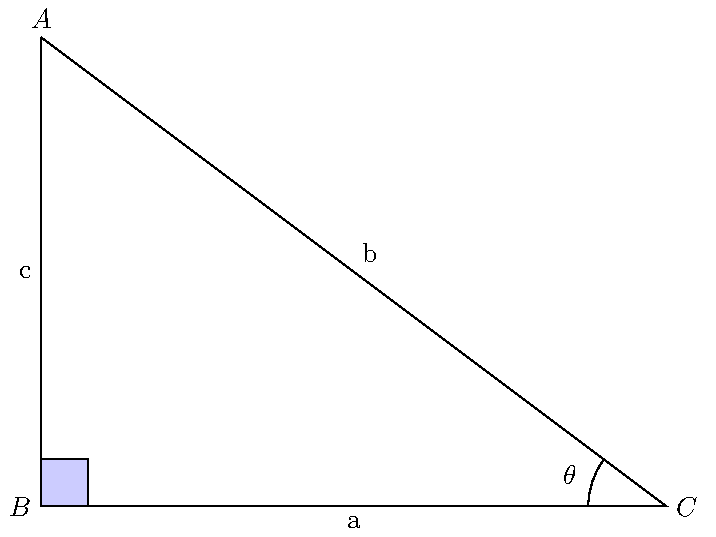
\includegraphics[width=0.6\columnwidth]{figs/trig_id/right/tri_right_angle.pdf}}
\caption{Right Angled Triangle}
\label{fig:tri_right_angle}	
\end{figure}
with angles $\angle A,\angle B$ and $\angle C$ and sides $a, b$ and $c$.  The unique feature of this triangle is $\angle B$ which is defined to be $90\degree$.
\item
	For simplicity, let the greek letter $\theta = \angle C$.  We have the following definitions.
\begin{equation}
\label{eq:tri_trig_defs}
\begin{matrix}
	\sin \theta = \frac{c}{b} & 	\cos \theta = \frac{a}{b} \\[1ex]
	\tan \theta = \frac{c}{a} & \cot \theta = \frac{1}{\tan \theta} \\[1ex]
	\csc \theta = \frac{1}{\sin \theta} & \sec \theta = \frac{1}{\cos \theta}
	\end{matrix}
\end{equation}
\item  
	\begin{equation}
	\cos \theta = \sin \brak{90\degree - \theta}
	\label{eq:tri_baudh_comp}	
	\end{equation}
\item
In  \figref{fig:tri_baudh}, 
show that 
%
\begin{equation}
\label{ch1_budh_basic}
b = a \cos \theta + c \sin \theta
\end{equation}
%
\begin{figure}[!ht]
	\begin{center}
		{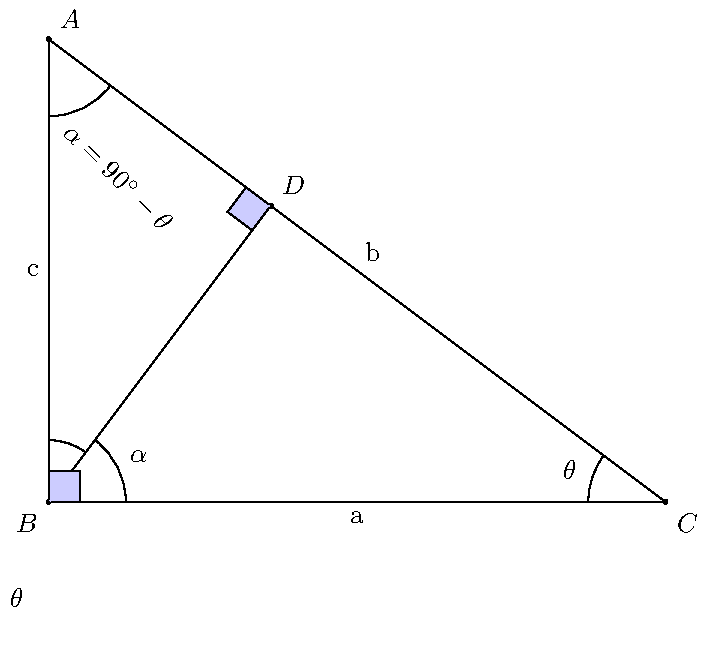
\includegraphics[width=0.6\columnwidth]{figs/trig_id/right/tri_baudh.pdf}}
	\end{center}
	\caption{Baudhayana Theorem}
	\label{fig:tri_baudh}	
\end{figure}
\solution We observe that
%
\begin{align}
CD &= a \cos \theta \\
AD &= c \cos\alpha = c \sin \theta \quad \brak{\text{From} \quad 
	\eqref{eq:tri_baudh_comp}	
	%\eqref{eq:tri_90-ang}
}
\end{align}
%
Thus,
\begin{equation}
CD + AD = b = a \cos \theta + c \sin \theta
\end{equation}
\item
From \eqref{ch1_budh_basic}, show that
%
\begin{equation}
%
\label{eq:tri_sin_cos_id}
\sin ^2 \theta + \cos ^2 \theta = 1
\end{equation}
%
\solution Dividing both sides of \eqref{ch1_budh_basic} by $b$, 
\begin{align}
1 &= \frac{a}{b}\cos\theta + \frac{c}{b}\sin\theta\\
\Rightarrow &\sin ^2 \theta + \cos ^2 \theta = 1 \quad \brak{\text{from} \quad \eqref{eq:tri_trig_defs}}
\end{align}
%
\item 
From \eqref{eq:tri_sin_cos_id}
\begin{align}
\label{eq:tri_sin_cos_minmax}
	\abs{\sin \theta} \le 1,\
	\abs{\cos \theta} \le 1
\end{align}
\item
	Using \eqref{ch1_budh_basic}, show that
	\begin{equation}
	\label{eq:tri_baudh}
	b^2 = a^2 + c^2
	\end{equation}
	\eqref{eq:tri_baudh} is known as the Baudhayana theorem.  It is also known as the Pythagoras theorem.
\\
\solution From \eqref{ch1_budh_basic},
\begin{align}
b &= a\frac{a}{b} + c \frac{c}{b} \quad \brak{\text{from} \quad \eqref{eq:tri_trig_defs}}\\
\implies b^2 &= a^2 + c^2
\end{align}
%
\item In a right angled triangle, the hypotenuse is the longest side.
\label{them:hyp_largest}
\\
\solution From 
	\eqref{eq:tri_baudh},
\begin{align}
	a \le b,\ c \le b.
\end{align}
\item $ABC$ is an isosceles triangle in which altitudes $BE$ and $CF$ are drawn to equal sides $AC$ and $AB$ respectively . Show that these altitudes are equal.
%
	\\
	\solution In $\triangle$s $BFC$ and $BEC$,
\begin{align}
	\label{eq:tri_isoc-alt}
	BF &= a \sin C,\
	CE = a \sin B 
	\\
	\implies BF &= CE, \because B = C.
\end{align}
\begin{figure}[H]
	\centering
		{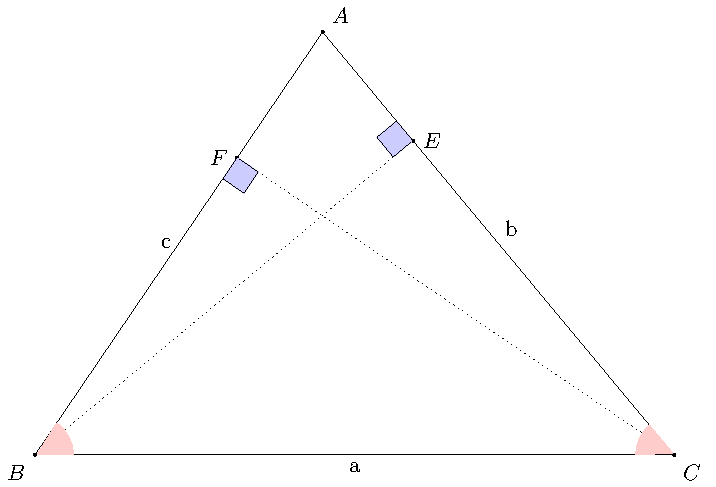
\includegraphics[width=0.6\columnwidth]{figs/trig_id/right/tri_isoc-alt.pdf}}
	\caption{$B = C$}
	\label{fig:tri_isoc-alt}
\end{figure}
\item $ABC$ is a triangle in which altitudes $BE$ and $CF$ to sides $AC$ and $AB$ are equal. Show that
%
$AB = AC$.
%
\\
\solution
	In \eqref{eq:tri_isoc-alt},
\begin{align}
	BE &= CF \implies 
	 a \sin C
	= a \sin B 
	\\
	\text{or, } B &= C
\end{align}
\item A ladder is placed against a wall such that its foot is at a distance of 2.5$m$ from the wall and its top reaches a window 6$m$ above the ground. Find the length of the ladder.
\item  A ladder 10$m$ long reaches a window 8$m$ above the ground. Find the distance of the foot of the ladder from base of the wall.
\item  A guy wire attached to a vertical pole of height 18$m$ is 24$m$ long and has a stake attached to the other end. How far from the base of the pole should the stake be driven so that the wire will be taut?
\item  An aeroplane leaves an airport and flies due north at a speed of 1000$km$ per hour. At the same time, another aeroplane leaves the same airport and flies due west at a speed of 1200$km$ per hour. How far apart will be the two planes after $1\frac{1}{2}$ hours?
\end{enumerate}
